% -*- TeX -*-

\documentclass[aspectratio=169]{beamer}

\usepackage{listings}
\usepackage{amsmath}
\usepackage{tikz}
\usetikzlibrary{shapes,calc}

\title{Crustal Deformation Modeling Tutorial}
\subtitle{Meshing with Complex Geometry}
\author{Charles Williams \\
  Brad Aagaard \\
  Matthew Knepley}
\institute{
\includegraphics[scale=0.4]{../../logos/cig_blackfg}}
\date{June 11, 2019}


% ---------------------------------------------------- CUSTOMIZATION
\renewcommand{\thispdfpagelabel}[1]{}
\usetheme{CIG}
% Style information for PyLith presentations.

% Colors
\definecolor{ltorange}{rgb}{1.0, 0.74, 0.41} % 255/188/105
\definecolor{orange}{rgb}{0.96, 0.50, 0.0} % 246/127/0

\definecolor{ltred}{rgb}{1.0, 0.25, 0.25} % 255/64/64
\definecolor{red}{rgb}{0.79, 0.00, 0.01} % 201/0/3

\definecolor{ltpurple}{rgb}{0.81, 0.57, 1.00} % 206/145/255
\definecolor{purple}{rgb}{0.38, 0.00, 0.68} % 97/1/175

\definecolor{ltblue}{rgb}{0.2, 0.73, 1.0} % 51/187/255
\definecolor{mdblue}{rgb}{0.28, 0.50, 0.80} % 72/128/205
\definecolor{blue}{rgb}{0.12, 0.43, 0.59} % 30/110/150

\definecolor{ltltgreen}{rgb}{0.7, 1.00, 0.7} % 96/204/14
\definecolor{ltgreen}{rgb}{0.37, 0.80, 0.05} % 96/204/14
\definecolor{green}{rgb}{0.23, 0.49, 0.03} % 59/125/8
  
\definecolor{dkslate}{rgb}{0.18, 0.21, 0.28} % 47/53/72
\definecolor{mdslate}{rgb}{0.45, 0.50, 0.68} % 114/127/173
\definecolor{ltslate}{rgb}{0.85, 0.88, 0.95} % 216/225/229


\newcommand{\includefigure}[2][]{{\centering\includegraphics[#1]{#2}\par}}
\newcommand{\highlight}[1]{{\bf\usebeamercolor[fg]{structure}#1}}
\newcommand{\important}[1]{{\color{red}#1}}
\newcommand{\issue}[2]{\item[Issue:] {\color{red}#1}\\{\item[Soln:] \color{blue}#2}\\[4pt]}

\setbeamercolor{alerted text}{fg=ltgreen}
\setbeamertemplate{description item}[align left]


\newcommand{\lhs}[1]{{\color{blue}#1}}
\newcommand{\rhs}[1]{{\color{red}#1}}
\newcommand{\annotateL}[2]{%
  {\color{blue}\underbrace{\color{blue}#1}_{\color{blue}\mathclap{#2}}}}
\newcommand{\annotateR}[2]{%
  {\color{red}\underbrace{\color{red}#1}_{\color{red}\mathclap{#2}}}}
\newcommand{\eqnannotate}[2]{%
  {\color{blue}%
  \underbrace{\color{black}#1}_{\color{blue}\mathclap{#2}}}}

\newcommand{\trialvec}[1][]{{\vec{\psi}_\mathit{trial}^{#1}}}
\newcommand{\trialscalar}[1][]{{\psi_\mathit{trial}^{#1}}}
\newcommand{\basisvec}[1][]{{\vec{\psi}_\mathit{basis}^{#1}}}
\newcommand{\basisscalar}[1][]{{\psi_\mathit{basis}^{#1}}}

\newcommand{\tensor}[1]{\bm{#1}}
\DeclareMathOperator{\Tr}{Tr}

\usefonttheme[onlymath]{serif}

% minted shortcuts
\newminted{cfg}{bgcolor=ltslate,autogobble,fontsize=\tiny}
\newminted{bash}{bgcolor=ltltgreen,autogobble,fontsize=\tiny}

% PyLith components
\newcommand{\pylith}[1]{{\ttfamily\color{magenta}#1}}



% --------------------------------------------------------- DOCUMENT
\begin{document}

% ------------------------------------------------------------ SLIDE
\maketitle

% ========================================================== SECTION
\section{Meshing}
\subsection{General steps}

% ------------------------------------------------------------- LOGO
\logo{
\includegraphics[height=4.5ex]{../../logos/cig_blackfg}}

% ------------------------------------------------------------ SLIDE
\begin{frame}
  \frametitle{Meshing Complex Geometry}
  \summary{Steps in creating a mesh}
  
  \begin{itemize}
  \item Determine geometric features needed
    \begin{itemize}
    \item Fault geometry
    \item Topography
    \item Sharp structural boundaries
    \item Magma sources with complex geometry
    \end{itemize}
  \item Create spline curve (2D) or NURBS surface (3D) in CUBIT/Trelis
  \item If using surface in several models export it for future use
  \item Use surfaces within CUBIT/Trelis to webcut or split
    volumes/surfaces
  \item Choose discretization according to type of problem
  \end{itemize}

\end{frame}

% ========================================================== SECTION
\subsection{Subduction meshing Example}

% ------------------------------------------------------------ SLIDE
\begin{frame}
  \frametitle{Meshing of a subduction zone}
  \summary{3-D coarse meshing of Cascadia with a simulated splay fault}
  
  \begin{itemize}
  \item Three-dimensional Cascadia subduction zone example\\
    \important{{\tt examples/3d/subduction/mesh}}
    \begin{itemize}
    \item Generate fault surfaces and export as ACIS files using
      \important{\tt generate\_surfjou.py} script to create
      \important{\tt geometry\_surfs.jou} file.
      \begin{itemize}
      \item Generate subduction interface from SLAB1.0 contours --
        script performs georeferencing to our local coordinates system
        as well as creating journal files.
      \item Generate slab bottom as an offset from subduction interface.
      \item Generate fictitious splay fault along a contour of subduction
        interface.
      \end{itemize}
    \item Generate volume geometry using \important{\tt geometry.jou}.
    \item Generate mesh using either \important{\tt mesh\_hex.jou} or
      \important{\tt mesh\_tet.jou}.
    \end{itemize}
  \end{itemize}


\end{frame}


% ========================================================== SECTION
\subsection{Problem geometry}

% ------------------------------------------------------------ SLIDE
\begin{frame}
  \frametitle{Simulated Cascadia Subduction Zone}
  \summary{Geometry with subduction thrust, slab and crust bottom, and
    splay fault}
 
  \vfill
  \begin{center}
    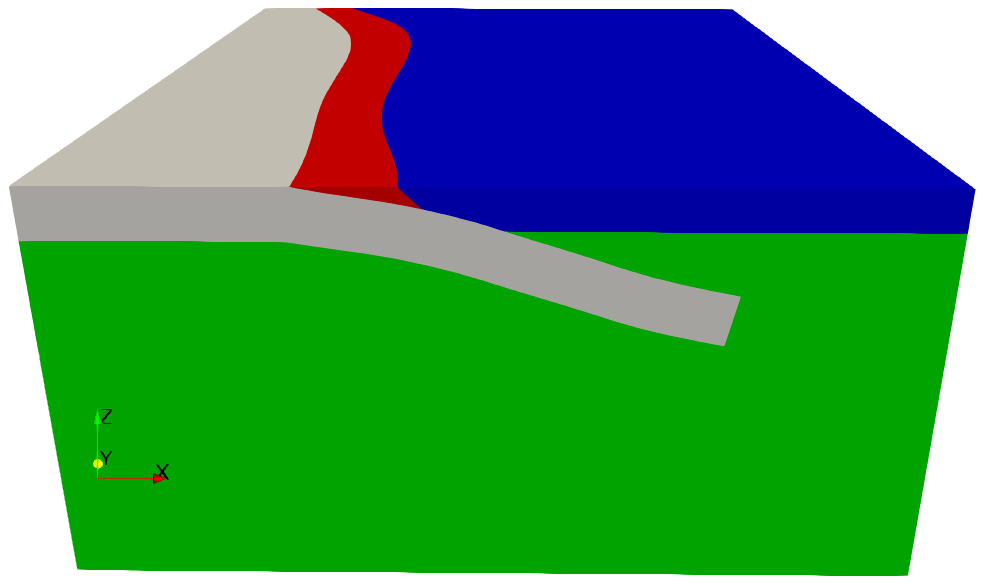
\includegraphics[height=6.1cm]{figs/subduction3d_conceptualmodel}
  \end{center}
  \vfill

\end{frame}


% ========================================================== SECTION
\subsection{Tetrahedral mesh}

% ------------------------------------------------------------ SLIDE
\begin{frame}
  \frametitle{Tetrahedral mesh generated for Cascadia problem}
  \summary{Constant resolution mesh with approximately 144k cells}
 
  \vfill
  \begin{center}
    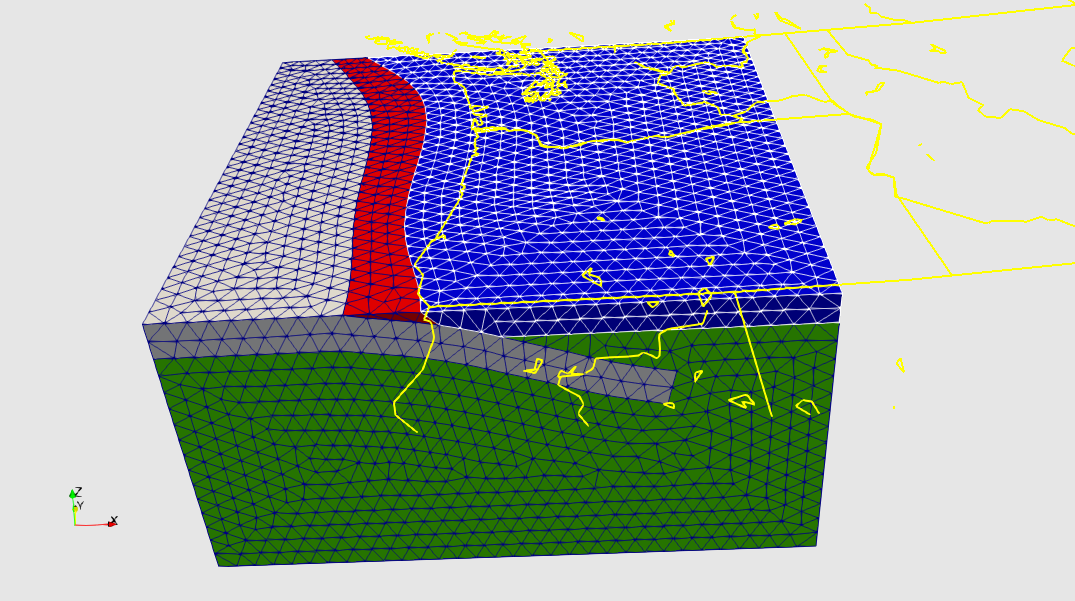
\includegraphics[height=6.1cm]{figs/subduction3d_tetmesh}
  \end{center}
  \vfill
 
\end{frame}


% ------------------------------------------------------------ SLIDE
\subsection{What's missing}

\begin{frame}
  \frametitle{What's missing}
  \summary{Additional modifications for real problems}
  
  \begin{itemize}
  \item Mesh needs to be larger to move boundaries away from region of
    interest.
    \begin{itemize}
    \item Enclose inner region in a larger box.
    \item Let Trelis/Cubit mesh internal surfaces (untested).
    \end{itemize}
  \item The mesh is much too coarse and not graded.
    \begin{itemize}
    \item Use sizing function to create a nicely graded mesh. See
      \important{\tt examples/meshing/cubit\_cellsize} for an example.
    \end{itemize}
  \end{itemize}

\vfill
NOTE:  If anyone does not have Cubit/Trelis, the mesh is available on the
PyLith wiki:
\important{https://wiki.geodynamics.org/software:pylith:cdm2019}
 
\end{frame}



% ======================================================================
\end{document}


% End of file
